\documentclass[11pt,a4paper]{article}
\usepackage{od,wrapfig,array}
\usepackage[utf8]{inputenc}
\usepackage[main=german,russian]{babel}

\pagestyle{headings}
\title{TRIZ Summit Cup – 2020/2021}
\setcounter{tocdepth}{2} 
\author{(Nicht autorisierte) Übersetzung ins Deutsche von Hans-Gert Gr\"abe,
  Leipzig} 
\date{4. Dezember 2020}

\begin{document}
\maketitle
\tableofcontents
\enlargethispage{12em}
\clearpage
\section{Kategorie 8-10 Jahre}

\subsection{Nomination „Erfinden“}

\subsubsection*{Aufgabe 1. Der Marsrover.}
Eine fantastische Geschichte beschreibt eine Expedition zum Mars.  Das
Raumschiff ging in einem Tal mit einer sehr unebenen Oberfläche herunter:
überall Hügel, Gruben, Steine. Die Astronauten rüsteten schnell ein
Geländefahrzeug aus -- ein Radfahrzeug mit großen aufblasbaren Reifen. Doch am
ersten Steilhang kippte der Geländewagen zur Seite. Und dann... Nein, leider
gab es in der Geschichte keinen Erfinder. Was denkst du: Was hätte er
vorgeschlagen? Beachte, dass die Astronauten nicht die Möglichkeit hatten, das
Geländefahrzeug umzubauen.  (Eine Aufgabe aus dem Buch von G.S. Altschuller
„Und dann kam der Erfinder“ -- \foreignlanguage{russian}{И тут появился
  изобретатель}. Eine Übersetzung des relevanten Ausschnitts aus dem Buch ist
diesen Materialien beigefügt).

Analysiere die Kontrolllösung (im Buch angegeben\footnote{Eine Übersetzung des
  hier erwähnten Fragments aus dem Buch ins Deutsche finden Sie bei den
  Wettbewerbsmaterialien.}): Finde das Konfliktpaar, formuliere den
Widerspruch, das IER, beschreibe, mit welchem Vorgehensmuster der Widerspruch
gelöst werden kann. Schlage andere Lösungen vor.

\subsubsection*{Aufgabe 2. Der Fahrer des Mondfahrzeugs.}
Du liebst Rennwagenmodelle mit Fernsteuerung fahren oder das Fahren auf einer
schwierigen Strecke im Fahrsimulator?  Jetzt stelle dir vor, du bist der
Fahrer eines Mondfahrzeugs, eines echten Transportmittels, das in der Lage
sind, auf dem Mond herumzufahren. Im November 1970 hat das unbemannte
Raumschiff „Luna 17“ den \emph{Lunochod} als erstes solches Fahrzeug auf dem
Erdtrabanten abgesetzt, um die Oberfläche des Mondes direkt zu untersuchen.
Die Steuerung des Lunochod übernahm eine Gruppe von 11 Personen in mehreren
Schichten, die aus folgenden Personen bestand: dem Kommandanten, dem Fahrer,
dem Antennenausrichter, dem Steuermann und dem Bordingenieur. Während der
Ausbildung der Fahrer auf dem Lunodrom entstand ein Problem -- der Lunochod
wurde ferngesteuert, d.h. der Fahrer sieht den Lunochod auf einem Bildschirm,
und die Kommandos, die er sendet, werden erst nach 3-5 Sekunden ausgeführt
(Laufzeit des Signals zum Mond und zurück sowie für die Signalverarbeitung) --
dies ist sehr ungewöhnlich für den Fahrer und erfordert ein langes Training.
Hier ist eine Episode des Trainings: „Die Motoren sind eingeschaltet. Der
Lunochod rückt vorwärts und bleibt gleich wieder stehen -- der Fahrer befahl
ihm zu stoppen, und die Maschine folgte dem Befehl.  Aber derMensch konnte
nicht erklären, warum er das Experiment abbrach -- ihm schien es, dass der
Lunochod sich seitwärts bewegte.  Die Telesteuerung war nicht so einfach.  Es
fehlte der Raum, an den die Augen so gewöhnt sind. Nach 15 Minuten stand der
Fahrer von seinem Sessel auf. Und obwohl der Raum ziemlich kühl war, konnte
man sein Hemd auswringen -- die Arbeit vor dem Bildschirm erforderte eine hohe
Anspannung. Nach mehreren Stunden am Bildschirm hatte sich der Fahrer an die
Situation „gewöhnt“, und der Lunochod folgte gehorsam, aber am nächsten Tag
fing alles wieder von vorne an -- die erlernten Fähigkeiten ware wieder
verloren gegangen“.  Die Situation ist klar: Die Fähigkeiten, den Lunochod
über Bildschirm zu steuern, sollten möglichst lange erhalten bleiben, aber es
ist unmöglich, die ganze Zeit auf der Trainingsstation zu verbringen. Was
schlägst du dem Lunochod-Fahrer vor, wie kann er in seinem normalen Leben
seine Fernsteuerfähigkeiten weiter verbessern?  Formuliere Widersprüche, das
IER, berücksichtige die verfügbaren Ressourcen.

\subsection{Nomination „Fantasieren“}

\subsubsection*{Aufgabe 1.}
In Arthur C. Clarkes Roman \emph{Rendevouz mit Rama} wird ein außerirdisches
Raumschiff beschrieben, das bis zu 50 Kilometer groß ist. Verwende die
„Zoom“-Technik und beschreibe das größte Raumschiff, das du dir vorstellen
kannst.

\subsubsection*{Aufgabe 2.}

Im Science-Fiction-Roman \emph{Das dritte Jahrtausend} von Heinrich Altov (dem
Schriftsteller-Pseudonym von G.S. Altschuller) wird beschrieben, wie Menschen
den Planeten Jupiter in Gas und Staub zermalmt haben (Anwendung des
TRIZ-Prinzips der „Zerlegung“). Es entstand eine riesige Gaswolke um die
Sonne, die so dicht ist wie die Atmosphäre der Erde. Man kann darin in
Düsen-Jets von Planet zu Planet fliegen und sogar mit Ballons. In der
interplanetaren Gaswolke entstehen Wolkengebilde und Wolken, es blitzt. Denke
dir eine Geschichte über die Abenteuer von Kindern aus, die mit einem Ballon
zum Mars reisen.

\subsection{Nomination „TRIZ-Werkzeuge“}

\subsubsection*{Aufgabe 1.}
Die Erkundung des Kosmos bringt aufregende Abenteuer, außergewöhnliche
Entdeckungen und Freude, das Unbekannte zu erkennen, mit sich. Diese
Forschungen haben auch rein praktische Anwendungen. Du weißt sicher, dass
Teflonbeschichtung, drahtlose Elektrowerkzeuge, Geolokalisierungsdienste und
viele andere Erfindungen, die unser Leben bequemer und sicherer machen, in der
Raumfahrtindustrie entstanden sind. Die Aufgaben in der Kategorie
„TRIZ-Werkzeuge“ sind mit solchen Erfindungen verbunden.

\begin{itemize}[noitemsep]
\item[1)] Lege einen Katalog „kosmischer Erfindungen“ an, die Einzug ins
  tägliche Leben gehalten haben.
\item[2)] Formuliere Widersprüche, die in diesem Erfindungen gelöst wurden. 
\item[3)] Schlage ungewöhnliche Anwendungen dieser Erfindungen für das Lösen
  noch nicht gestellter Aufgaben vor.
\end{itemize}

\subsubsection*{Aufgabe 2.}

Märchen, Mythen, Legenden sind oft der einzige Weg, um herauszufinden, wie sie
unsere fernen Vorfahren gelebt haben. Und es ist so interessant, was auf
unserer Erde vor vielen Jahrhunderten geschah, welche Geschichten erzählt
wurden, wie die Häuser aussahen, was unsere Vorfahren gedacht und geträumt
haben. Und möchtest du nicht auch, dass über deine Familie, deine Freunde,
deine Stadt Menschen nach vielen Tausend Jahren erfahren?  Denke dir ein
Märchen, Mythos, Legende, fantastische Geschichte aus, die so interessant ist,
dass sie auch noch nach Hunderten von Jahren erzählt wird.

\subsection{Nomination „Forschung“}

\subsubsection*{Aufgabe 1.}

\newcommand{\AnimalsInCosmos}{Seit den Anfängen der Erforschung des Weltraums
  wurde der Mensch von Tieren begleitet (und manchmal ersetzt). In den mehr
  als 60 Jahren Weltraumforschung sind alle möglichen Arten von Tieren sind im
  Weltraum gewesen. Die interessantesten Experimente im Orbit stehen im
  Zusammenhang mit der Kultivierung von Pflanzen. Es war nicht sofort möglich,
  Bedingungen zu schaffen, unter denen die Pflanzen nicht nur grüne Masse
  ansetzten, sondern auch blühten und Früchte trugen. Hier also das
  Forschungsthema: „Tiere und Pflanzen im Weltraum“.  Du kannst für deine
  Untersuchungen ein spezifischeres Thema wählen.
\begin{itemize}[noitemsep]
\item Katalog „Tiere im Weltraum“. Art der Tiere, Datum des Fluges ins All,
  Dauer des Aufenthalts im Weltraum, Ziele des Experiments, Ergebnisse des
  Experiments.
\item Katalog „Pflanzen im Weltraum“. Art der Pflanze, Datum des Fluges ins
  All, Dauer des Aufenthalts im Weltraum, Ziele des Experiments, Ergebnisse
  des Experiments.
\item Katalog „Geräte zur Aufrechterhaltung der Lebenstätigkeit von Tieren im
  Kosmos“.  Welche Aufgaben standen und wie wurden diese in jedem der Geräte
  gelöst?
\item Katalog „Geräte zur Aufrechterhaltung der Lebensaktivität von Pflanzen
  im Kosmos“.  Welche Aufgaben standen und wie wurden diese in jedem der
  Geräte gelöst?
\item Welche Aufgaben der Anpassung von Tieren und Pflanzen an den Aufenthalt
  im Weltraum sind immer noch ungelöst?  Schlage mögliche Lösungen vor.
\end{itemize}}

\AnimalsInCosmos

\subsection{Nomination „TRIZ-Videos“}

\newcommand{\VideoOne}{Gibt es in deiner Stadt Orte, die mit der Erforschung
  des Kosmos in Zusammenhang stehen?  Erstelle einen Bericht über einen
  Museumsbesuch, eine Ausstellung, eines Wissenschaftszentrums. Versuche,
  Raumfahrt-Experten zu ihren Kosmosforschungen zu befragen. }

\newcommand{\VideoTwo}{Illustriere mit den Mitteln Film oder Animation, wie
  erfinderische Probleme gelöst werden. Lasse dir eine Geschichte einfallen,
  in der ein Problem auftritt, versuche, im Detail zu kommentieren, worin der
  Widerspruch besteht, welche ideale Lösung erreicht werden soll und welche
  Techniken zur Lösung verwendet werden.}

\newcommand{\GeneralText}{Die Videos sollten kurz sein (2 bis 10 Minuten).
  Alle Autoren des Videos müssen angegeben werden: der Autor des Drehbuchs,
  der Operator, der Cutter, die Schauspieler, usw.  Diese Arbeit soll auf die
  Erstellung von methodischem Material für die TRIZ-Ausbildung abzielen. Auf
  der Website des TRIZ-Summit sind Videos veröffentlicht, die für den letzten
  TRIZ Summit Cup eingereicht wurden: \\
  \url{http://triz-summit.ru/ru/contest/competition/video/}\\
  \url{https://www.youtube.com/channel/UCjMNOjboWRBQA72DJvaC7ew/featured}

  An der Vorbereitung der Aufgaben des TRIZ Summit Cups 2020/2021 waren
  M.S. Rubin und N.V. Rubina beteiligt, die Nominierung „Fantasieren“ wurde
  von P.R. Amnuel' vorbereitet.}

\subsubsection*{Aufgabe 1.}\VideoOne
\subsubsection*{Aufgabe 2.}\VideoTwo

\GeneralText
\clearpage

\section{Kategorie 11-14 Jahre}

\subsection{Nomination „Erfinden“}

\subsubsection*{Vorbemerkung. Die weiche Marslandung.}

\begin{wrapfigure}{r}{.3\textwidth}\vspace*{-1em}\centering
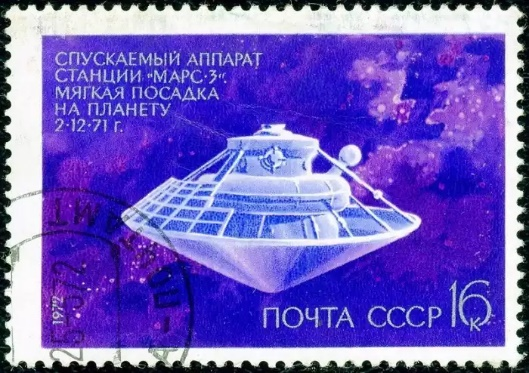
\includegraphics[width=.25\textwidth]{jEMlaM.jpg}
\end{wrapfigure}
Der Traum vieler Weltraumforscher bleibt ein Flug zum Mars. Das erste
künstliche Objekt, das die Oberfläche des Roten Planeten berührte, war der
Marsrover PROP-M\footnote{Die Abkürzung steht für die russischen Worte
  \foreignlanguage{russian}{Прибор оценки проходимости - Марс}, Gerät zur
  Beurteilung der Geländegängigkeit auf dem Mars.}. Am 2. Dezember 1971
erfolgte die weiche Landung.  Versuchen wir, einen Teil des Weges zum Mars
samt Landeanflug, den Marsrover und Überlegungen seiner Konstrukteure
nachzuvollziehen. Die Landekapsel hat also die Grenzen der Marsatmosphäre
erreicht, es beginnt die aerodynamische Bremsung.  Für die weiche Landung wird
ein Fallschirmsystem verwendet.

\subsubsection*{Aufgabe 1.}
Um ein Fallschirmsystem zu starten, wird ein Auswurf-Fallschirm verwendet --
er ist klein, schafft aber die notwendige Zugkraft für eine vollständige
Öffnung der Hauptfallschirme. Der Auswurf-Fallschirm darf sich nicht früher
oder später als in dem Moment öffnen, in dem die Landekapsel in die
Marsatmosphäre eintritt. Was könnte als Signal zur Aktivierung des
Zündtriebwerks an der Hülle des Auswurf-Fallschirms dienen?  (Formuliere das
IER und suche die erforderlichen Ressourcen)
\begin{center}
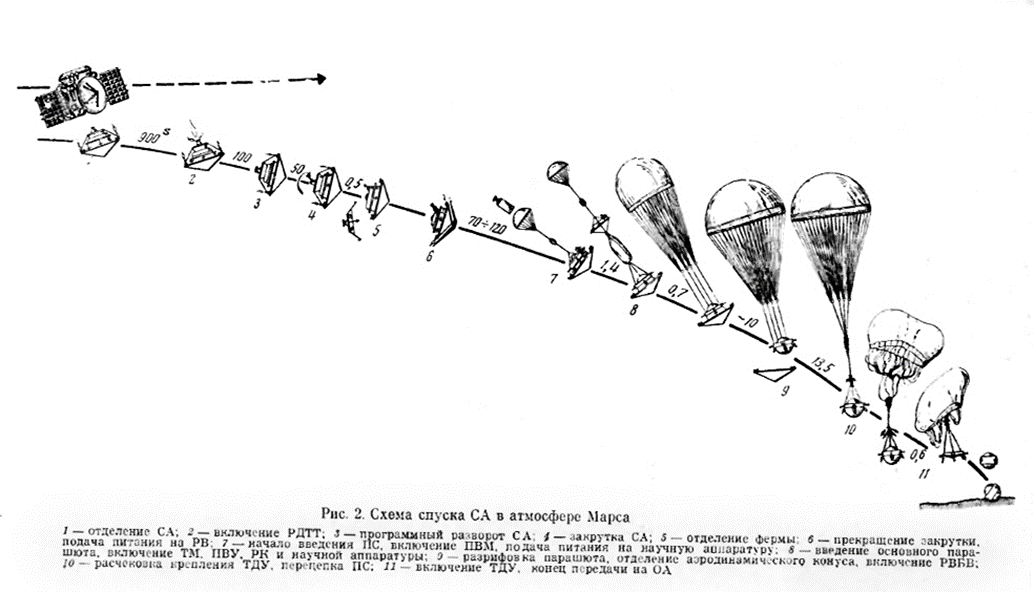
\includegraphics[width=.95\textwidth]{12uaYg.png}
\end{center}

\subsubsection*{Aufgabe 2.}
Der nächste Schritt besteht darin, den Hauptfallschirm zu aktivieren und zu
öffnen. Es ist dabei mehrere Operationen umzusetzen: Öffnen des
Fallschirmfachs, Entfernen des oberen Deckels, den Hauptfallschirm vollständig
zu öffnen und schließlich zu verhindern, dass der Hauptfallschirm die
Landekapsel am Boden überdeckt. Analysieren Sie das Bremssystem der
Landekapsel, identifizieren Sie alle unerwünschten Wirkungen, die beim Bremsen
auftreten können, formulieren Sie diese Widersprüche. Welche Konstruktionen
können an der Beseitigung dieser unerwünschten Wirkungen beteiligt werden?
\begin{center}
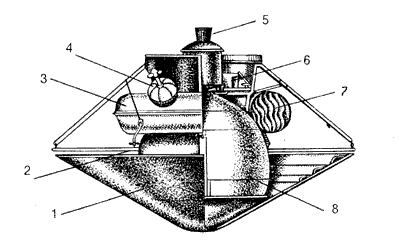
\includegraphics[width=.4\textwidth]{GIj0Ml.png}\hfill
  \begin{minipage}[b]{.55\textwidth}\small
    Landekapsel der Station Mars-2:
    \begin{itemize}[noitemsep]
    \item[1] -- aerodynamischer Kegel;
    \item[2] -- Antenne des Funkhöhenmessers;
    \item[3] -- Fallschirmcontainer;
    \item[4] -- Antrieb des Deckels des Auswurf-Fallschirms;
    \item[5] -- Antrieb zur Steuerung der Landekapsel;
    \item[6] -- Instrumente und Apparate des Steuerungssystems;
    \item[7] -- Hauptfallschirm;
    \item[8] -- automatische Marsstation
    \end{itemize}
  \end{minipage}
\end{center}
Diese Geschichte hat eine unerwartete und interessante Fortsetzung.

\subsubsection*{Aufgabe 3.}
Sie haben sich noch nie gefragt, was über gebrauchte Apparate bekannt ist, die
auf dem Mond, dem Mars oder der Venus zurückgeblieben sind?  Die Erforschung
der Resultate vernünftiger Aktivitäten auf den Planeten und ihren Satelliten
hat sich noch nicht zu einer eigenständigen Domäne entwickelt, aber
Publikationen zur „Weltraumarchäologie“ gibt esw schon recht viele.  Man
könnte denken, dass die Landeplätze aller Apparate, die Planeten und deren
Satelliten erkundet haben, genau bekannt, aber... Vitaly Yegorov beschreibt
diese Aufgabe so: „Als ich mir die Website von \emph{HiRise}\footnote{High
  Resolution Imaging Science Experiment} anschaute, fand ich nur ein Bild aus
dem Jahr 2007 mit dem Titel \emph{Center of Soviet Mars 3 Landing Ellipse}.
Das war für mich eine Entdeckung, weil ich mir der Allmacht von NASA und
HIRise so sicher war, dass ich erwartet hatte, eine genaue Angabe vorzufinden,
wo diese Station steht.  Eine kurze Suche im Internet ergab ebenfalls kein
Ergebnis. Es war also offensichtlich, dass Mars-3 nie gefunden worden war. Ich
lud das Foto im Vollformat (1.3 GB) herunter, öffnete es und verstand, warum
in fünf Jahren niemand die Station gefunden hat. (Das Bild hat eine Auflösung
von 30 cm pro Pixel, d.h. ein Objekt der Größe von 30 cm entspricht einem
Punkt.  Mars-3 ist ein 1.5\,m großes Objekt -- im Bild ein Objekt aus
$6\times6$ Pixeln). Stellen Sie sich eine Suche eines abgerundeten, 1.5 Meter
breites Objekts in einem Rechteck von $6\times20$ Kilometern vor.  Ich weiß,
viele Leute dachten sofort daran, dass man ein Programm schreiben muss, das
nach der Station sucht. Aber ich glaube nicht, dass eine Suche ohne KI möglich
ist. Ja, das Programm könnte interessante Felsblöcke von angemessener Größe
hervorheben.  Aber da gibt es Tausende solcher Objekte, denn in der Nähe
befindet sich ein Krater, aus dem fächerförmig Steine flogen.“

Was würden Sie in dieser Situation vorschlagen? Wie finden Sie Mars-3? Und die
Hauptsache ist, warum überhaupt die Ergebnisse intelligenter menschlicher
Aktivitäten auf Planeten und Satelliten erforschen, welche Informationen
können wir erhalten?

\subsubsection*{Aufgabe. Der gefährliche Planet.}
Eine fantastische Geschichte beschreibt einen erstaunlichen Planeten. Alles
darauf ist wie auf der Erde: die gleiche Atmosphäre, die gleichen Pflanzen und
Tiere. Aber die Insekten und Vögel fliegen mit Überschallgeschwindigkeit.
Lassen Sie uns nicht näher darauf eingehen, wie sie das tun.  Das ist nicht
der Punkt. Sie wissen wahrscheinlich, dass eine Flugzeugkollision mit Vögeln
zu Unfällen führt. Aber hier ist die Luft gefüllt mit lebendigen „Kugeln“ und
„Granaten“...  Es wurden zwei Astronauten auf dem Planetebn abgesetzt, und man
schaffte es gerade noch, sie zu retten. Sogar ein gepanzertes Geländefahrzeug
wurde schnell von Überschallfliegen zerstört...  Stellen Sie sich vor, Sie
wären auf der Expedition zu diesem Planeten. Machen Sie Vorschläge, wie Sie
und die Besatzung in Sicherheit zu bringen sind.

Stellen wir uns die umgekehrte Situation vor. Auf dem Planeten, den wir
untersuchen, wurde es intelligentes Leben entdeckt. Die Geschwindigkeit der
Veränderung, die Reaktionsgeschwindigkeit der intelligenten Wesen ist jedoch
im Vergleich zu Menschen viele Male verlangsamt. So langsam, dass ein Moment
für einen Menschen für die Wesen auf dem fremden Planeten Jahre
dauert\footnote{HGG: Eigentlich ist es umgekehrt -- ein Moment für die fremden
  Wesen dauert mehrere Menschenjahre.}. Wie stellt man Kontakt her, wie
verhandelt man?

\subsection{Nomination „Fantasieren“}

\subsubsection*{Aufgabe 1.}
Heutzutage gehen Astronauten in Raumanzügen ins All, die es ihnen erlauben, zu
atmen und die sie vor Strahlung schützen. Kann eine Person im Kosmos ohne
Raumanzug leben? Bisher nicht wirklich, noch nicht, aber
Fantasy-Schriftsteller haben darüber geschrieben, wie es klappen könnte.
Denken auch Sie sich etwas aus. Nutzen Sie dabei einen der Tricks der
TRIZ-Phantasietechnik.

\subsubsection*{Aufgabe 2.}
In Hal Clements Roman \emph{Unternehmen Schwerkraft} spielt sich die Handlung
auf einem Planeten ab, auf dem die Schwerkraft 800 Mal so groß ist wie auf der
Erde.  Denke dir einen fantastischen Planeten aus, der sich von der Erde durch
einen anderen Parameter unterscheidet. Beschreibe die Abenteuer einer
Raumschiffbesatzung auf einem Planeten wie diesem.

\subsection{Nomination „TRIZ-Werkzeuge“}

\subsubsection*{Aufgabe 1.}

\newcommand{\CosmicInventions}{Kosmische Reisen und Forschungen ist ein Traum
  vieler Generationen mutiger Menschen. Diese Forschungen haben auch rein
  praktische Anwendungen. Sie wissen sicher, dass die Teflon-Beschichtung,
  drahtlose Elektrowerkzeuge, Geolokalisierungsdienste und viele andere
  Erfindungen, die unser Leben komfortabler und sicherer machen, in der
  Kosmos-Industrie gemacht wurden. Die Aufgaben in der Nomination
  „TRIZ-Werkzeuge“ sind genau mit solche Erfindungen verbunden.
\begin{itemize}[noitemsep]
\item[1)] Stellen Sie einen Katalog von „Weltraum-Erfindungen“ zusammen, die
  Anwendungen im Alltag fanden.
\item[2)] Formulieren Sie die Widersprüche, die mit diesen Erfindungen gelöst
  wurden.
\item[3)] Schlagen Sie eine ungewöhnliche Verwendung dieser Erfindungen zur
  Lösung von noch nicht gestellten Aufgaben vor.
\end{itemize}}

\CosmicInventions

\subsection{Nomination „Forschung“}

\subsubsection*{Aufgabe 1.}

\AnimalsInCosmos

Ist es möglich, im Orbit ähnliche Bedingungen zu schaffen wie in komplexen
natürlichen Systemen wie z.B. einem Wald, einer Wiese, usw., wo Tiere und
Pflanzen miteinander interagieren?  Gibt es solche Projekte bereits,
welche Probleme haben sich bei  deren Realisierung ergeben?  

\subsubsection*{Aufgabe 2.}
In jeder Familie gibt es Geschichten, die von Generation zu Generation
weitergegeben werden: vom Großvater, der von Chicago nach Russland kam, von
seiner Großmutter, die Leben an der Front gerettet hat, usw. Es gibt tragische
Fälle, es gibt komische Fälle, aber man erinnert sich an sie wegen ihrer
Klarheit, sie werden gern viele Male wiedererzählt, werden vom Vater zum Sohn
weitergegeben. Um die wahren Geschichten wachsen legendäre Details.
Beschreiben Sie die Geschichte Ihrer Familie: seit wann und woher Ihre Familie
stammt, welche besonderen Taten Ihre Vorfahren vollbracht haben, welche
besonderen Geschichten haben Ihre Familie begleitet. Schreiben Sie das auf,
was Sie über Ihre Familie mitteilen möchten.  Wenn Sie die Geschichte über
Ihre Familie beendet haben, geben Sie einen Kommentar zu der Geschichte ab.
stellen Sie sich vor, Ihre Geschichte würde im 25. Jahrhundert gelesen, und
man weiß dort nichts anderes über unserer Zeit. Wie wird unsere Zivilisation
in deren Augen aussehen, wenn sie nur auf der Grundlage Ihrer
Familiengeschichte studiert würde? Was würden Sie in Ihrer Geschichte
verändern, damit sie von den Menschen auch nach vielen Jahrhunderten
verstanden wird?

\subsection{Nomination „TRIZ-Videos“}
\subsubsection*{Aufgabe 1.}\VideoOne
\subsubsection*{Aufgabe 2.}\VideoTwo

\GeneralText
\clearpage

\section{Kategorie 15-17 Jahre}

\subsection{Nomination „Erfinden“}

\newcommand{\Aberration}{Es ist bekannt, dass sich das gebrochene Sonnenlicht
  in ein Spektrum zerlegt. Die Astronomen haben sehr darunter gelitten. In den
  Linsen des Teleskops wird auch das Licht von Sonne, Planeten und Sternen
  gebrochen. Und kosmische Objekte sind von bunten Auren umgeben, was daran
  hindert, sie richtig zu beobachten. Dieses Phänomen wird als „chromatische
  Aberration“ bezeichnet. Der große englische Physiker I. Newton hielt es für
  unmöglich, sie loszuwerden.  Schlagen Sie eine Methode zur Herstellung von
  Linsen vor, die keine chromatische Aberration verursachen.}

\newcommand{\CosmicOperation}{Obwohl nur starke und gesunde Menschen als
  Kosmonauten akzeptiert werden, kann in den Raumstationen der nahen Zukunft
  viel mit ihnen passieren. Es ist möglich, dass eine komplizierte Operation
  erforderlich wird. Auf der Erde wird der Patient auf den Operationstisch
  gelegt, wo sowohl der Patient als auch der Tisch, die Instrumente und Ärzte
  durch die Schwerkraft in ihrer Position gehalten werden. Aber in der
  Schwerelosigkeit ist das nicht so einfach. Auf den ersten Blick kann ein
  Tisch an den Boden geschraubt werden. Aber Ärzten kann man nicht
  festschrauben. Sie müssen sich bewegen. Auch die Instrumente und die
  Behälter mit Präparaten kann man nicht verschrauben. Auch den Kranken kann
  man nicht immer festbinden -- er könnte dabei weitere Verletzungen erleiden.
  Und wenn die Operation schwerwiegend ist, eine umfassende Öffnung des
  Körpers erfordert, müssen auch die inneren Organe vom „Fliegen“ abgehalten
  werden.  Schlagen Sie einen Entwurf für den Operationssaal vor,
  Operationstisch, Werkzeuge und Vorrichtungen für die unterschiedlichsten
  Operationen in der Schwerelosigkeit.}

\subsubsection*{Aufgabe 1.}\Aberration
\subsubsection*{Aufgabe 2.}\CosmicOperation

\subsection{Nomination „Fantasieren“}

\subsubsection*{Aufgabe 1.}

In G. Altshullers \emph{Etagenschema}\footnote{Siehe zu dieser grundlegenden
  Technik in der TRIZ-Fantastik die deutsche Übersetzung eines Texts von
  P. Amnuel in den Wettbewerbsmaterialien.} gibt es vier Arten („Etagen“), um
eine neue fantastische Idee zu entwickeln. Studieren Sie dieses Schema.
Denken Sie sich Ideen der dritten und vierten Etage für das Objekt „Raumanzug“
aus und beschreiben Sie diese.


\subsubsection*{Aufgabe 2.}

In Larry Nivens fantastischem Roman „Integral Trees“ leben die Menschen auf
einen Planeten, der ein riesiger Baum ist, der im Weltraum auf einem Orbit um
einen Stern kreist, der wie die Sonne aussieht. In Paul Sheffields Roman „Die
Welt ist ein Ring“ leben die Menschen auf der Oberfläche eines riesigen Rings,
der sich um einen Stern dreht.  Denken Sie sich einen fantastischen Planeten
aus und beschreiben Sie ihn, nutzen Sie dazu eine beliebige
Fantasietechnik. Schreiben Sie eine kleine Abenteuergeschichte auf dem
Planeten, den Sie erfunden haben.

\subsection{Nomination „TRIZ-Werkzeuge“}

\newcommand{\BlackBox}{Formulieren Sie mit Hilfe einer morphologischen Tabelle
  (siehe dazu den Text von M.S. Rubin zur „Black Box der
  Zivilisation“\footnote{Eine deutsche Übersetzung dieses Textes finden Sie
    bei den Wettbewerbsmaterialien.}) ein Forschungsthema, eine Teilaufgabe
  für die „Black Box der Zivilisation“. Sammeln Sie Beispiele und Aufgaben zum
  Thema Ihrer Wahl. Analysieren Sie die gesammelten Informationen.  Welche
  Wege der Informationsweitergabe über die moderne Zivilisation können Sie
  anbieten?  Was kann, nach Ihrer Meinung, heute getan werden, um
  Informationen über unsere der Zivilisation zu erhalten?}

\subsubsection*{Aufgabe 1.}\BlackBox
\subsubsection*{Aufgabe 2.}\CosmicInventions

\subsection{Nomination „Forschung“}

\newcommand{\BlackBoxOfCivilization}{
  \subsubsection*{Aufgabe zur „Black Box der Zivilisation“.}
(zitiert nach: G.S. Altshuller, I.M. Vertkin, „Wie wird man ein Häretiker?“
  Petrosawodsk, 1991, S. 166-168).
  \begin{quote}
Moderne Großraumflugzeuge haben eine so genannte „Black Box“ eingebaut. Sie
ist für die Aufzeichnung der Flugmodi vorgesehen. Im Falle einer Havarie sind
deren Gründe so leicht herauszufinden und die Schuldigen zu identifizieren.
Wenn der Unfall Schuld der Piloten war oder durch Unzulänglichkeiten der
Flugzeugkonstruktion hervorgerufen wurde, ermöglicht die Analyse der
Aufzeichnungen, zukünftige Flüge sicherer zu machen. Eine Havarie verhindern
oder den Opfern des Unglücks helfen kann die „Black Box“ nicht, das ist aber
auch nicht Teil ihrer Funktion. Ihr Hauptziel ist die Arbeit für „morgen“; die
„Black Box“ ermöglicht es, aus fremden Fehlern zu lernen. 

In letzter Zeit wurden auch Ozeanschiffe mit diesen Geräten ausgerüstet.
Offensichtlich werden „Black Boxes“ in naher Zukunft obligatorisch in allen
Arten öffentlicher Verkehrsmittel werden, und möglicherweise auch in privaten
Kraftfahrzeugen.

Zu allen Zeiten haben Menschen, die sich auf gefährliche Reisen begaben oder
sich auf tragische Ereignisse vorbereiteten, versucht, ihren Nachkommen ihre
Erfahrungen, ihre Beschreibungen des Vorgefallenen weiterzugeben. Gewöhnlich
wurden solche Aufzeichnungen in tragischen Zeiten von Menschen gemacht: in
belagerten Städten, in Gefängnismauern, in Erwartung des baldigen Todes.
Erinnern Sie sich an die Qumran-Manuskripte, das Tagebuch der Polarexpedition
von Scott, Aufzeichnungen der Selbstbeobachtung von Alain Bombard.

In der Regel werden solche „Vermächtnisse“ erst im letzten Moment begonnen,
wenn der Mangel an Zeit und geeigneten Bedingungen bereits gravierend ist.
Deshalb kennen wir nur einige wenige Aufzeichnungen, die auf wundersame Weise
überlebt haben. Auf alles muss man sich rechtzeitig vorbereiten, darunter auch
(oder vielleicht an erster Stelle) auf Katastrophen.

Unsere Erde ist nicht weniger verwundbar als jedes andere „öffentliche
Verkehrsmittel“. In früheren Zeiten galten als Ursache für ein „Weltende“
mystische über\-irdische Kräfte. In der jüngeren Vergangenheit wurde diese
Rolle an mysteriöse Außerirdische übergeben, die den Erdlingen feindlich
gesonnen sind.  Heute heißt es, dass unser größter Feind wir selbst sind, und
es werden genetische, soziale, demographische, atomare, ökologische und Krisen
vergleichbarer Art vorausgesagt. Eigentlich spielt es keine Rolle, aus welchem
Grund es zu einer Katastrophe kommen kann, aus diesen oder noch nicht
bekannten Gründen; das Wichtigste ist, dass dies grundsätzlich möglich ist.
Die Erde braucht also ihre eigene „Black Box“. Sie muss die wahren Ursachen
der möglichen Tragödie aufzeichnen, die Aufzeichnungen über die erforderliche
Zeit intakt halten und an künftige Generationen weitergeben: solche
Erfahrungen, insbesondere so negative und globale, sind von unschätzbarem
Wert.

Nur die Zukunft kann die Frage nach der heutigen Aktualität einer „Black Box“
für den Planeten eindeutig beantworten.  Eines kann man getrost schon heute
sagen: das Problem ist kein Fantasieprodukt. Wenn es nicht „brennt“, gut, dann
haben wir Zeit, uns ruhig und sorgfältig auf eine Lösung vorzubereiten. Wenn
die Zeit knapp ist, dann müssen wir das tun, was wir noch tun können. Kurz
gesagt, je früher die Arbeit an diesem Problem beginnt, desto besser.

Die Lösung des Problems hängt weitgehend vom Ausmaß der wahrscheinlichen
Katastrophe ab. Ein paar mögliche Varianten:
\begin{itemize}[noitemsep]
\item[a)] Die Hälfte der Weltbevölkerung verschwindert infolge der
  Katastrophe.  Verbindungen zwischen Städten bleibt erhalten. Bis zu einem
  gewissen Grad bleibt die frühere Infrastruktur erhalten.
\item[b)] Auf der Erde verbleiben mehrere zehntausend Menschen. Verbidungen
  wird es praktisch keine geben. Die Reste der Bevölkerung degradieren
  ziemlich schnell, zu primitiven Handwerken, zu primitiven Techniken. Es
  dauert lange, bis die Voraussetzungen für einen spürbaren Sprung nach vorn
  wieder gegeben sein.
\item[c)] Intelligentes Leben wird vom Angesicht der Erde verschwinden. In
  100-150 Jahren wird es Bedingungen geben, die für menschliches Leben
  akzeptabel sind, aber wann die Wiedergeburt des Geistes erfolgt, „das weiß
  allein Allah“.
\item[d)] Alles Leben verschwindet von der Erde. Die Zeit, um solche
  Bedingungen wieder herzustellen, ist eine Milliarde Jahre.
\end{itemize}
Konzentrieren wir uns auf die schwierigste, die letzte Option. Wenn wir uns
etwas einfallen lassen, um einen verschärften Konflikt zu überwinden, dann
wird die Aufgabe unter weicheren Bedingungen um so mehr gelöst werden können.

Also, die Bedingungen des Problems. In 100-150 Jahren verschwindet alles Leben
auf der Erde. Die mögliche Erholungszeit beträgt eine Milliarde Jahre.
\textbf{Wie kann man eine „Black Box“ über eine solche zeitliche Distanz
  weitergeben? Was soll hineingeschrieben werden?}

Dies sind sehr schwierige Fragen. Zum Beispiel die Frage nach der
Übertragungs\-technik von Informationen. Schließlich weiß man heute noch
nicht, wem die Informationen übergeben werden muss.  weiß, welches Aussehen
intelligentes Leben eine Milliarde Jahre nach unserer Ära hat... Ja und wird
es von selbst auf der Erde entstehen? Wie kann man bei der Wiederherstellung
intelligenten Lebens helfen? Wie kann der Genpool unserer Flora und Fauna
erhalten werden? Wie stellt man es an, dass die Informationen rechtzeitig zur
Verfügung steht: wenn sie bereits in der Lage sind, herauszufinden, um was die
Rede geht, und es noch nicht zu spät ist? Wie schaffen wir es, dass Sie
Informationen ohne Mühe entschlüsseln können? Wie kann eine Aufzeichnung über
eine solche zeitliche Entfernung erhalten werden?  Wie stellt man es an, dass
die Informationen geglaubt und nicht als dummer Witz abgetan wird?

Nicht klarer ist die Frage nach dem Inhalt der „Black Box“. Wahrscheinlich mus
der „Kasten“ aus zwei Teilen bestehen: einem „operativen“ (über die Ursachen
der Havarie) und einem „stationären“ (über akkumulierte Kultur und Wissen über
die Erde). Wie kann man den „operativen“ Teil ständig auffüllen, den
unmittelbaren Moment und die nachfolgende Zeit eigeschlossen? Was sollte in
den „stationären“ Teil geschrieben werden? „Alles Wissen der Welt“? Was genau?
Was sind die Auswahlkriterien?  Welche Empfehlungen können wir dem zukünftigen
intelligenten Leben weitergeben, um ähnliche Tragödien zu verhindern?

Es gibt viele Fragen...

Warum ist das ein gutes Problem? „Übermittlung von Informationen“ ist heute
ein Thema für Erstentdecker, völlig frei von Konkurrenz, zumindest für die
nächsten 30-50 Jahre (wir hoffen, dass sich die Vernunft dennoch durchsetzen
wird, und die Menschheit sich der Problems früherer Katastrophe bewusst wird).
Dies ist eine der wenigen Themen, die völlig frei von einer negativen Seite
sind.  Das Thema ist maximal edel, gesellschaftlich äußerst nützlich, von
einem Super-Großformat.  Es ist bereits heute offensichtlich, dass dies ein
lebenslanges Thema ist, und nicht nur für eines. Das Thema hat soziale und
technische Aspekte, d.h. es ist geeignet für Menschen mit beliebigen
Spezialisierungen.

(Ein typischer scheinheiliger Einwand gegen dieses Problem lässt sich im
Voraus vorhersagen: Wenn ein Haus brennt, muss man nicht aufschreiben, was den
Brand verursacht hat, sondern Eimer mit Wasser heranschleppen. Eine mögliche
Katastrophe der Zivilisation wirft viele Probleme auf, die meisten von ihnen
werden heute noch sehr abstrakt wahrgenommen. Die Mehrheit der Bevölkerung des
Planeten arbeitet weiterhin in den Unternehmen seiner Staaten, d.h. beteiligt
sich weiterhin an der Zerstörung der Natur. Nur wenige schlagen die Glocke und
versuchen, die Flammen zu löschen. Aber niemand, nicht ein einizger Mensch auf
der ganzen Erde, ist dem Black-Box-Problem nahe gekommen! Wer weiß, vielleicht
ist ein Brief, der eine Milliarde Jahre in die Zukunft gerichtet ist,
wichtiger als zwei Eimer Wasser heute ...).
  \end{quote}

Siehe hierzu auch das Arbeitsmaterial von M.S. Rubin \emph{Kurze Analyse des
  Problems der „Black Box einer Zivilisation“}, das in deutscher Übersetzung
diesen Wettbewerbsmaterialien beiliegt.
}

\BlackBoxOfCivilization

\subsection{Nomination „TRIZ-Videos“}

\newcommand{\VideoThree}{Illustrieren Sie mit Film- oder Animationswerkzeugen
  die Lösung erfinderischer Probleme. Das können sowohl technische Lösungen
  sein als auch Erfindungen auf nicht-technischen Gebieten. }

\subsubsection*{Aufgabe 1.}\VideoOne
\subsubsection*{Aufgabe 2.}\VideoThree

\GeneralText
\clearpage

\section{Kategorie Studenten}

\subsection{Nomination „Erfinden“}

\subsubsection*{Aufgabe 1.}\Aberration
\subsubsection*{Aufgabe 2.}\CosmicOperation

\subsection{Nomination „Fantasieren“}

\subsubsection*{Aufgabe 1.}

In Greg Egans Romanzyklus „Das orthogonale Universum“ spielt sich die Handlung
in einem Universum ab, in dem die Lichtgeschwindigkeit von der Wellenlänge
abhängt. Denekn Sie ein Universum aus und beschreiben es, in dem ein anderes
physikalisches Gesetz oder Weltkonstante geändert wurde.

\subsubsection*{Aufgabe 2.}
Der Romanzyklus von Stephen Baxter und Terry Pratchett „Die lange Erde“
beschreibt Welten, von denen jede eine Erde hat, die sich von unserem Planeten
dadurch unterscheidet, dass die Entwicklung irgendwann in einem Stadium der
Evolution anders verlaufen ist als in unserer Realität. In einem Fall sind die
Dinosaurier nicht ausgestorben, in einem anderen Fall war der ganze Planet mit
Wäldern bedeckt, in einem dritten gibt es keine Menschen, aber es gibt
intelligente Hunde... Denekn Sie sich einen kosmischen Faktor aus, der einst
den Lauf der Evolution auf der Erde veränderte, und beschreiben Sie, wie es
auf dem Planeten als Ergebnis der Auswirkungen dieses Faktors heutzutage
aussieht.

\subsection{Nomination „TRIZ-Werkzeuge“}

\subsubsection*{Aufgabe 1.}\BlackBox
\subsubsection*{Aufgabe 2.}\CosmicInventions

\subsection{Nomination „Forschung“}

\BlackBoxOfCivilization

\subsection{Nomination „TRIZ-Videos“}

\subsubsection*{Aufgabe 1.}\VideoOne
\subsubsection*{Aufgabe 2.}\VideoThree

\GeneralText
\end{document}
